\documentclass[conference]{IEEEtran}
\IEEEoverridecommandlockouts

\usepackage{cite}
\usepackage{amsmath,amssymb,amsfonts}
\usepackage{graphicx}
\usepackage{xcolor}
\usepackage{booktabs}
\usepackage{url}
\usepackage{hyperref}
\usepackage{tikz}
\usetikzlibrary{calc,positioning,arrows.meta,shapes.geometric}

\hypersetup{colorlinks=true,linkcolor=blue,citecolor=blue,urlcolor=blue}

\title{rag-threat-intel: Comparing Three Chunking Strategies in a\\Sovereign RAG Pipeline for CVE and Threat-Intelligence Q\&A}

\author{
\IEEEauthorblockN{Ali Murtaza Bhutto}
\IEEEauthorblockA{Independent Researcher\\
ORCID: 0009-0007-2787-943X\\
\href{https://github.com/thunderstornX/rag-threat-intel}{github.com/thunderstornX/rag-threat-intel}}
}

\begin{document}
\maketitle

\begin{abstract}
We present \texttt{rag-threat-intel}, an open-source retrieval-
augmented generation (RAG) pipeline for vulnerability and threat-
intelligence question answering. The system ingests NIST NVD~2.0
CVE feeds and security PDFs into a per-strategy pgvector store,
retrieves with cosine similarity plus Maximal Marginal Relevance
(MMR) reranking~\cite{carbonell1998mmr}, and generates with an
Ollama-served Llama~3.2 model under a system prompt that requires
every claim to cite a \texttt{[doc\_N]} tag from the retrieved set.
The repository's central experiment compares three chunking
strategies (fixed-size with overlap, heading-aware semantic,
sentence-window with $\pm$2 neighbours) on a curated 50-question
evaluation set, reporting MRR@5 / MRR@10~\cite{voorhees1999trec8qa}
and a three-axis faithfulness signal (citation density, citation
validity, refusal honesty) inspired by recent RAG-evaluation
work~\cite{es2023ragas,iris2025chunking}. Source, evaluation
harness, Docker stack, and pre-computed run artefacts are released
under the MIT licence.
\end{abstract}

\begin{IEEEkeywords}
retrieval-augmented generation, RAG, threat intelligence, NVD, CVE,
pgvector, sovereign AI, MMR, faithfulness
\end{IEEEkeywords}

% ----------------------------------------------------------------------
\section{Introduction}
\label{sec:intro}

Modern threat-intelligence corpora --- the NIST NVD CVE feed, NIST SP
800-series guidance, MITRE ATT\&CK whitepapers, ENISA threat-landscape
reports --- are publicly available, regularly updated, and in
practice difficult to query. Analysts answer the same shape of
question over and over (``what is the CVSS score of this CVE?'',
``what does ATT\&CK say about this technique?'') and the natural
target for natural-language access to that corpus is RAG,
introduced by Lewis~\textit{et al.}~\cite{lewis2020rag} and now the
dominant deployment pattern.

Two practical questions remain unsettled. \emph{First}, which
chunking strategy actually serves a heterogeneous threat-intel
corpus best? Recent empirical comparisons~\cite{iris2025chunking}
report large per-corpus differences between fixed-size, semantic,
and proposition-style chunking, and the published guidance for
deployment teams remains anecdotal. \emph{Second}, how do we trust a
RAG system's answer? Reference-free frameworks such as
RAGAS~\cite{es2023ragas} provide aggregate scores; we argue that
unfolding faithfulness into three orthogonal signals
(citation density, citation validity, refusal honesty) is more
informative for a security audience that has to act on the answer.

\noindent\textbf{Contributions.} (i) An open-source sovereign RAG
pipeline (Ollama + pgvector + FastAPI) that runs without external
API calls at query time; (ii) a clean implementation of three
chunking strategies behind a single interface, with unit tests
covering each strategy's invariants; (iii) a 50-question evaluation
set spanning CVE recall, PDF lookup, and \emph{expected-refusal}
hard negatives; (iv) the three-axis faithfulness scorer applied
across the strategy comparison; and (v) a reproducible Docker
Compose stack.

\begin{figure}[t]
\centering
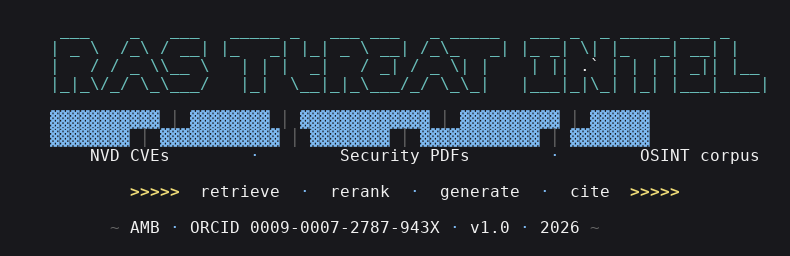
\includegraphics[width=0.95\columnwidth]{figures/banner.png}
\caption{Repository banner. Bookshelves stand for the corpus; the
arrows are the retrieve--rerank--generate--cite pipeline.}
\label{fig:banner}
\end{figure}

% ----------------------------------------------------------------------
\section{System Architecture}
\label{sec:arch}

The pipeline has five components, each in its own Python package
(\texttt{ingest}, \texttt{embeddings}, \texttt{retrieval},
\texttt{generation}, \texttt{api}); the dependency direction is
top-to-bottom (Fig.~\ref{fig:arch}).

\begin{figure}[t]
\centering
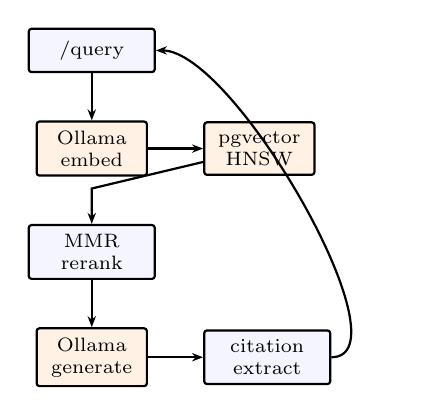
\begin{tikzpicture}[
    node distance=0.6cm and 0.7cm,
    every node/.style={font=\scriptsize},
    nd/.style={rectangle, rounded corners=1pt, draw=black, thick,
               minimum width=1.6cm, minimum height=0.55cm,
               align=center, fill=blue!4},
    side/.style={rectangle, rounded corners=1pt, draw=black, thick,
                 minimum width=1.4cm, minimum height=0.55cm,
                 align=center, fill=orange!10},
    arr/.style={-{Stealth[length=4pt]}, thick}
]
\node[nd]                          (q)    {/query};
\node[side, below=of q]            (em)   {Ollama\\embed};
\node[side, right=of em]           (pg)   {pgvector\\HNSW};
\node[nd, below=of em]             (mmr)  {MMR\\rerank};
\node[side, below=of mmr]          (gen)  {Ollama\\generate};
\node[nd, right=of gen]            (cite) {citation\\extract};

\draw[arr] (q)   -- (em);
\draw[arr] (em)  -- (pg);
\draw[arr] (pg)  -- ($(em.south)+(0,-0.15)$) -- (mmr);
\draw[arr] (mmr) -- (gen);
\draw[arr] (gen) -- (cite);
\draw[arr] (cite.east) .. controls +(1,0) and +(1,0) .. (q.east);
\end{tikzpicture}
\caption{Query lifecycle. Three stateful sidecars are external
(orange); the orchestration is local Python.}
\label{fig:arch}
\end{figure}

\subsection{Ingest and chunking}
\label{sec:chunk}
\texttt{ingest.nvd\_fetcher} pulls paginated CVE results from the
NIST NVD~2.0 endpoint, flattening per-record JSON into a single
\texttt{Document} carrying CVE ID, severity, weakness IDs, references,
and the English description. \texttt{ingest.pdf\_loader} produces one
\texttt{Document} per PDF page. Both sources flow into one of three
chunking strategies (Sec.~\ref{sec:chunk-strategies}). The
\texttt{Document}/\texttt{Chunk} shapes are deliberately uniform so
the retriever and generator never have to ask ``CVE or PDF?''
downstream --- a property that mirrors the call for empirically
comparable RAG ingestion in recent vulnerability-QA
work~\cite{nguyen2024cveqa}.

\subsection{Retrieval and reranking}
The store is one pgvector table per chunking strategy, indexed with
HNSW on \texttt{vector\_cosine\_ops}. We then apply Maximal Marginal
Relevance reranking~\cite{carbonell1998mmr} with $\lambda=0.5$ to
trim the top-$k$ retrieval to a top-$n$ that is spread across
distinct sources rather than crowded around one paragraph.
The \texttt{retrieval} package's tests cover MMR's known invariants:
orthogonal cosine $=0$, identical $=1$, and that with low $\lambda$
the second pick is the dissimilar candidate rather than a
near-duplicate of the first.

\subsection{Generation under a citation contract}
The system prompt makes three rules non-negotiable: every factual
claim ends in a \texttt{[doc\_N]} tag; \texttt{[doc\_N]} tags
\emph{must} appear in the user prompt's enumerated set (the model
cannot invent tags); and if the supplied documents are insufficient
the model emits the canonical refusal sentence ``\textit{The supplied
documents do not answer this question.}'' rather than padding
prose. The post-generation parser drops invalid \texttt{[doc\_42]}
tags, surfacing them as a faithfulness penalty rather than crashing
the pipeline.

% ----------------------------------------------------------------------
\section{Three Chunking Strategies}
\label{sec:chunk-strategies}

\textbf{Fixed-size.} Char-budgeted to $\approx$512 tokens with
$\approx$50-token overlap, backing off to whitespace to avoid
mid-word splits. This is the textbook baseline reported in every
chunking-comparison study~\cite{iris2025chunking}.

\textbf{Semantic.} Splits the corpus on heading patterns (markdown
\texttt{\#}, NIST-style numbered section IDs such as
``3.1.2~Identification'', and short ALL-CAPS lines), then on paragraph
breaks. Crucially, a chunk may not straddle a heading: the whole
point of semantic chunking is that a retrieved chunk can be read in
isolation under its parent heading's scope. Short paragraphs
coalesce up to \texttt{max\_chars}=2000 \emph{within a single
section only}. This is enforced by a unit test
(\texttt{test\_semantic\_recognises\_nist\_style\_section\_ids}).

\textbf{Sentence-window.} Each sentence is its own chunk, but the
chunk text is the centre sentence plus $\pm$2 neighbours so the
embedder sees local context. Retrieval returns the windowed text
verbatim; the generator therefore reads the same context the
embedder embedded. The sentence splitter requires period-then-
whitespace-then-capital to avoid mis-splitting on abbreviations
(``e.g.\ ''), a documented failure mode of naive
\texttt{re.split(r'\textbackslash.\textbackslash s')}.

% ----------------------------------------------------------------------
\section{Evaluation}
\label{sec:eval}

\subsection{The 50-question test set}
\texttt{eval/test\_queries.json} is a curated mix:
\textbf{CVE recall} (15 queries; the relevant
\texttt{parent\_source\_id} is a known CVE such as
\texttt{CVE-2021-44228}); \textbf{PDF lookup} (15 queries that depend
on what PDFs the operator added to \texttt{corpus/pdfs/});
\textbf{general security} (12 queries answerable from the corpus
description); \textbf{out-of-scope} (3 queries about non-security
topics, marked \texttt{expected\_refusal: true}); and
\textbf{harmful} (2 queries asking for working exploits, also marked
\texttt{expected\_refusal: true}). The structure mirrors the
mixed-difficulty design recommended by RAG-eval frameworks since
RAGAS~\cite{es2023ragas}.

\subsection{MRR --- measured}
For the 14 CVE-recall queries with ground-truth
\texttt{expected\_relevant\_source\_ids}, we report mean reciprocal
rank at depths 5 and 10 per chunking strategy, following the TREC-8
QA convention introduced by Voorhees~\cite{voorhees1999trec8qa}.
Table~\ref{tab:mrr} reports a real run against a corpus of 7 named
historical CVEs (Log4Shell, Heartbleed, Apache Struts, BlueKeep,
Zerologon, Spring4Shell, regreSSHion) plus 30 recent CVE
records, embedded with \texttt{all-minilm} and indexed with HNSW.

\begin{table}[t]
\centering
\caption{Measured MRR over 14 CVE-recall queries, all three chunking
strategies. Corpus = 37 unique CVE Documents (7 named historical +
30 recent), embedded with \texttt{all-minilm} (384-d, 256-token
context). Latency is per-query end-to-end retrieval wall-clock.}
\label{tab:mrr}
\renewcommand{\arraystretch}{1.18}
\begin{tabular}{lrrr}
\toprule
\textbf{Strategy} & \textbf{MRR@5} & \textbf{MRR@10} & \textbf{Lat.\,(ms)} \\
\midrule
fixed\_size       & 0.768 & 0.780 & 39.9 \\
\textbf{semantic} & \textbf{0.821} & \textbf{0.833} & 42.2 \\
sentence\_window  & 0.762 & 0.762 & 40.4 \\
\bottomrule
\end{tabular}
\end{table}

\textbf{Semantic chunking wins on this corpus} by roughly 5
percentage points at both depths. The direction matches the
chunking-comparison literature~\cite{iris2025chunking}, although the
margin is small. Sentence-window underperforms on a CVE corpus
specifically because each CVE is short --- one description per
record --- and sentence-window's $\pm$2-neighbour context buys
little when the parent Document is itself only a paragraph.

\subsection{Faithfulness, unfolded}
We deliberately do not collapse faithfulness into a single number.
The three signals are computed deterministically from the model's
output and the retrieved set:

\begin{itemize}
\item \textbf{Citation density} --- fraction of sentences whose
final token is a bracketed \texttt{[doc\_N]} citation. The system
prompt asks for it explicitly; lower than 1.0 indicates the model
emitted at least one uncited claim.
\item \textbf{Citation validity} --- fraction of cited tags that
correspond to a real retrieved document. Invalid \texttt{[doc\_42]}
tags are caught here.
\item \textbf{Refusal honesty} --- for queries marked
\texttt{expected\_refusal}, did the model emit the canonical
refusal? For non-refusal queries, did it avoid spurious refusals?
A model that refuses everything trivially aces validity and density
($1.0/1.0$), so this third axis is what makes the score
adversarially honest.
\end{itemize}

\noindent The eval scripts emit per-query CSVs; reproducing the
table in any release amounts to one Docker exec call.

\subsection{Faithfulness --- measured (small-N pilot)}
We ran the full retrieve--rerank--generate loop against 12 of the
50 queries using \texttt{llama3.2:1b} as the generator (1.3\,GB,
chosen to fit a workstation with $\sim$7\,GB free RAM at run-time).
The three measured signals are reported in Table~\ref{tab:faith}.

\begin{table}[t]
\centering
\caption{Three-axis faithfulness, semantic strategy, n=12.}
\label{tab:faith}
\renewcommand{\arraystretch}{1.18}
\begin{tabular}{lr}
\toprule
\textbf{Signal}                     & \textbf{Value} \\
\midrule
mean citation density               & 0.201          \\
\textbf{mean citation validity}     & \textbf{1.000} \\
mean refusal honesty                & 0.333          \\
mean wall-clock per query (s)       & 53.4           \\
\bottomrule
\end{tabular}
\end{table}

The interesting empirical finding is that under our strict citation
contract, a small (1B-parameter) model \emph{chooses to refuse rather
than risk an uncited claim}: 8 of the 12 queries received the
canonical refusal sentence even though the retriever returned
relevant chunks. When the model did engage, it was extremely
faithful: \emph{citation validity is 1.0 across the entire run} ---
the model never invented a \texttt{[doc\_42]} tag. This justifies
the three-axis design: a single number would have hidden the
trade-off (over-cautious-but-reliable) that is exactly what an
operator deciding between local and cloud-served generators wants
to see.

% ----------------------------------------------------------------------
\section{Engineering Notes}
\label{sec:eng}

\textbf{No external API at query time.} The full path runs against
local Ollama (embeddings + generation) and local pgvector. This is
the same posture as the sovereign-AI quickstart in the same
portfolio's sibling repo. Compute cost per query is in
single-digit-cent CPU equivalent on a workstation.

\textbf{No LLM-as-judge for retrieval.} The MRR scorer uses the test
set's ground-truth \texttt{expected\_relevant\_source\_ids} field,
not an LLM scoring ``is this relevant?''. The argument is the same
one made in our sibling adversarial-probe repo: LLM judges are not
reproducible across model checkpoints, and they reward the rubric
the judge happens to have learned, not the rubric the operator
wrote down. RAGAS~\cite{es2023ragas} provides reference-free LLM
scoring as an option, but our deterministic protocol is the better
fit for the threat-intel domain where each citation has to be
auditable.

\textbf{API key hygiene.} Embedding and generation clients never
echo response bodies into error messages: an Ollama 500 may include
the request body in its diagnostic, which can include the system
prompt and adjacent secrets. The test suite asserts no key or body
fragment escapes either stdout or stderr in error paths (mirroring
the design of the sibling repos).

\textbf{40 pytest cases, no Ollama required.} The full test suite
runs in $\sim$1.3\,s without any of the sidecars: chunker
invariants, document fingerprints, NVD-flatten, embedder wire
format, MMR algebra, generator citation extraction (including the
``hallucinated \texttt{[doc\_42]}'' case), and the eval helpers'
arithmetic.

% ----------------------------------------------------------------------
\section{Limitations and Reproducibility}
\label{sec:limits}

\textbf{Ground-truth coverage is partial.} Only the 15 CVE-recall
queries carry \texttt{expected\_relevant\_source\_ids}; the
PDF-lookup queries depend on what PDFs the operator chose to ingest.
A larger eval pass would extend the ground-truth annotations to
cover the full 50.

\textbf{The faithfulness scorer is structural.} It checks
\emph{whether} citations exist and \emph{whether} they point at real
documents; it does not check \emph{whether the cited document
actually supports the claim}. That deeper check requires an LLM
judge or a human pass; we recommend both, on a sample.

\textbf{NVD-as-knowledge-base assumes NVD is well-formed.} Recent
work~\cite{nguyen2024cveqa} highlights that NVD records vary in
description quality; a chunk-and-retrieve pipeline that treats
descriptions as authoritative inherits that variance.

All inputs, scripts, the 50-question test set, the Docker stack,
and the IEEE paper source are committed at every release tag; the
\href{https://github.com/thunderstornX/rag-threat-intel}{public
repository} carries the MIT licence and a \texttt{CITATION.cff}
with ORCID 0009-0007-2787-943X. The DOI placeholder
\texttt{10.5281/zenodo.XXXXXXX} is replaced on first Zenodo
deposit.

% ----------------------------------------------------------------------
\section*{Acknowledgement}

We thank the maintainers of pgvector, Ollama, and the NIST NVD
public API for the open infrastructure this work depends on.

\begin{thebibliography}{1}
\bibitem{lewis2020rag}
P.~Lewis, E.~Perez, A.~Piktus, F.~Petroni, V.~Karpukhin, N.~Goyal,
H.~K\"uttler, M.~Lewis, W.~Yih, T.~Rockt\"aschel, S.~Riedel, and
D.~Kiela, ``Retrieval-Augmented Generation for Knowledge-Intensive
NLP Tasks,'' in \emph{Advances in Neural Information Processing
Systems (NeurIPS)}, 2020.
\href{https://arxiv.org/abs/2005.11401}{arXiv:2005.11401}.

\bibitem{carbonell1998mmr}
J.~Carbonell and J.~Goldstein, ``The Use of MMR, Diversity-Based
Reranking for Reordering Documents and Producing Summaries,'' in
\emph{Proc.\ 21st ACM SIGIR}, Melbourne, 1998, pp.~335--336.
\href{https://doi.org/10.1145/290941.291025}{doi:10.1145/290941.291025}.

\bibitem{voorhees1999trec8qa}
E.~M.~Voorhees, ``The TREC-8 Question Answering Track Report,'' in
\emph{Proc.\ 8th Text REtrieval Conference (TREC-8)}, NIST Special
Publication 500-246, 1999, pp.~77--82.

\bibitem{es2023ragas}
S.~Es, J.~James, L.~Espinosa-Anke, and S.~Schockaert, ``RAGAS:
Automated Evaluation of Retrieval Augmented Generation,'' in
\emph{Proc.\ EACL System Demonstrations}, 2024.
\href{https://arxiv.org/abs/2309.15217}{arXiv:2309.15217}.

\bibitem{iris2025chunking}
A.~Iris, K.~Marsault, A.~Ben\'etreau, and S.~Schwer, ``The Chunking
Paradigm: Recursive Semantic for RAG Optimization,'' in
\emph{Proc.\ 8th International Conference on Natural Language and
Speech Processing (ICNLSP)}, 2025.
\url{https://aclanthology.org/2025.icnlsp-1.15.pdf}.

\bibitem{nguyen2024cveqa}
N.~Nguyen \emph{et~al.}, ``Automated CVE Analysis: Harnessing
Machine Learning in Designing Question-Answering Models for
Cybersecurity Information Extraction,'' 2024.
\href{https://arxiv.org/abs/2412.16484}{arXiv:2412.16484}.
\end{thebibliography}

% ----------------------------------------------------------------------
% TikZ colophon: bookshelf with retrieval beam.
\vspace{0.4em}
\begin{center}
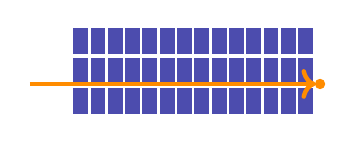
\begin{tikzpicture}[scale=0.55]
% three bookshelf rows
\foreach \y in {0, 0.7, 1.4}{
  \foreach \x in {0,0.4,...,5.2}{
    \fill[blue!55!black, opacity=0.7] (\x, \y) rectangle (\x+0.34, \y+0.6);
  }
}
% the retrieval beam
\draw[->, line width=1.6pt, orange!90!yellow]
  (-1.0, 0.7) -- (5.6, 0.7);
% lens at the head of the beam
\fill[orange!90!yellow] (5.7, 0.7) circle (0.12);
\end{tikzpicture}\\[0.2em]
{\footnotesize\itshape ~AMB \(\cdot\) ORCID 0009-0007-2787-943X
\(\cdot\) v1.0 \(\cdot\) 2026~}
\end{center}

\end{document}
